% Checked with Grammarly - 22/03/2021

\chapter{Implementation}

% =========================================

This chapter discusses the various implementation stages of the VisiBot Processing System and Interactive Web Application development and deployment. Such sections define the technologies, architectural design patterns, development practices, and deployment strategies used throughout the development process.

\section{Distributed Real-time Processing System}

\subsection{Message-based task queues with Celery and Redis}

Written in Python 3.9 \citep{Python39}, the VisiBot Processing System utilises several internal and external modules, services, and frameworks to create a flexible and reliable analysis system based on the Message Broker design pattern. I chose the Python programming language primarily due to the extensive availability of open-source community libraries, including various web development frameworks, API wrappers, and data analytic tools.

One such library used is Celery \citep{Celery}, a python-based asynchronous task queuing framework modelled on the Message Broker design pattern. Redis \citep{Redis} is an open-source data structure store commonly used for databasing, caching, and message brokering. It is used conjunction with Celery to enable the processing of vast amounts of messages across distributed worker instances. Through the queuing of programmatic tasks as messages, high quantities of synchronous, or otherwise, time-consuming tasks are actively consumed by Celery workers through interaction with a central broker system. Celery supports integration with various message brokers, including RabbitMQ, Amazon SQS, Redis, and Zookeeper. Within the context of this project, Redis was chosen as the primary message broker for VisiBot.

Celery tasks are created by an application and routed, stored, and eventually consumed through a broker system by a cluster of Celery workers. These workers can be distributed across several systems and configured automatically based on the queue's size and workload. Celery workers also support the execution of tasks in parallel. This enables the swift and concurrent execution of time-consuming tasks, which might otherwise bottle-neck synchronous applications. The VisiBot Processing System utilises Celery workers to analyse, identify, and extract botnet malware samples from honeypot sources and analyse them within automated sandbox environments. As this process can be time-consuming on synchronous systems, the adoption of a Message Broker design pattern through Celery and Redis ensures that analysis tasks are completed concurrently and reliably.

Flower, a python-based Celery monitoring tool by \citet{CeleryFlower} offers a remotely accessible web application dashboard, which allows for the monitoring task queues, celery workers, and successful or failed tasks. As the stack traces for all unsuccessful tasks are logged by Celery, such traces are remotely accessible through accessing the Flower dashboard, allowing for a convenient method for identifying and debugging worker run-time exceptions from within a deployed environment. The flower web interface has been protected with user authentication, as it allows users to remotely manage workers and view potentially confidential information, such as stack traces. A screenshot of the dashboard is shown below:

\begin{figure}
    \centering
    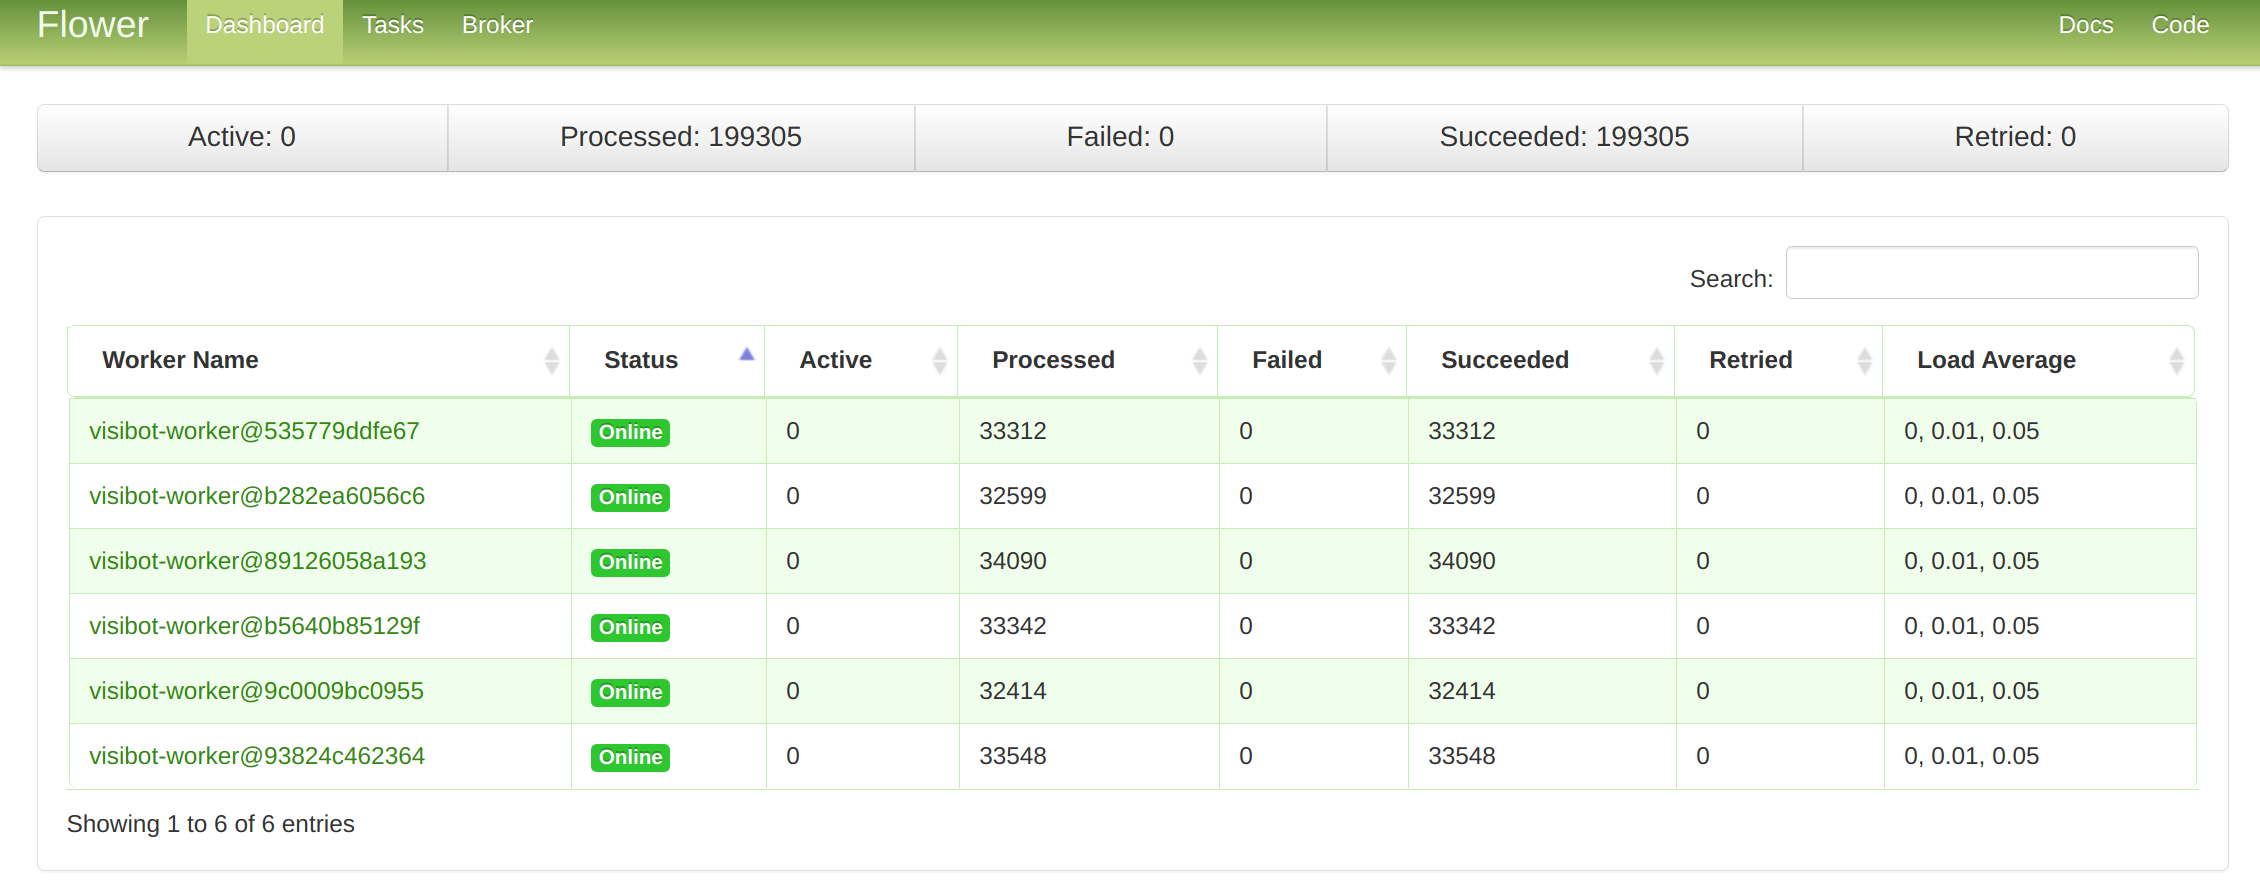
\includegraphics[width=1.0\linewidth]{images/flower-panel.png}
    \caption{Flower Dashboard. Celery workers are represented in a table as rows.}
    \label{fig:flower_dashboard} 
\end{figure}

\subsection{Docker}

As the proposed system utilises various applications, celery workers, servers, and external services, the setup and deployment process can introduce many complexities and anomalies due to various environmental factors such as different operating system, package managers, and system architecture. Thus, to streamline the setup and deployment process, all applications, workers, and services utilised by VisiBot have been encapsulated within a multi-container Docker application using the command-line tool Docker Compose \citep{DockerCompose}. 

A unique feature provided by Docker is that of image scalability. By containerising a single celery worker within a docker image, it can dynamically be scaled to allow multiple celery workers' instantaneous creation. The number of workers is scaled by appending the \texttt{docker-compose} command with the \texttt{--scale worker N} argument. For example, running the docker application with the argument \texttt{--scale worker 10} will prompt Docker to create 10 VisiBot Celery worker containers. Each container will initialise a new celery worker instance and connect to the Redis broker service, which is also containerised within a docker image. All other services and applications used by the VisiBot workers and processing system have also been containerised, including a locally accessible tor server, honeypot result scheduling system, Flask Web API, MaxMind GeoIP2 Updater, and a remotely accessible instance of Flower. Docker also enables shared access to storage between multiple containers through the creation of containerised volumes. Additionally, an \texttt{.env} file has been populated with a set of default environment variables. It is automatically read by docker-compose upon initialisation, allowing the user to change pre-defined aspects of the processing system, such as API keys and paths, without directly modifying any of the code.

As VisiBot workers use shared MaxMind GeoIP2 databases \citep{MaxMind} during analysis tasks, a shared volume was created such that the VisiBot workers could query a shared database hosted within the GeoIP container. Upon initialisation, the GeoIP creates a Cron-job using \texttt{crontab} \citep{Crontab} which, executes a GeoIP2 updating utility every week. This utility writes the latest versions of all MaxMind GeoIP2 databases to \texttt{/usr/local/share/GeoIP2}. By modifying the docker configuration of VisiBot's \texttt{docker-compose.yml}, this path was defined as a shared path accessible to all workers. A visualisation of the relationships between all docker containers within the VisiBot Processing System is shown below:


\begin{figure}[!htb]
    \centering
    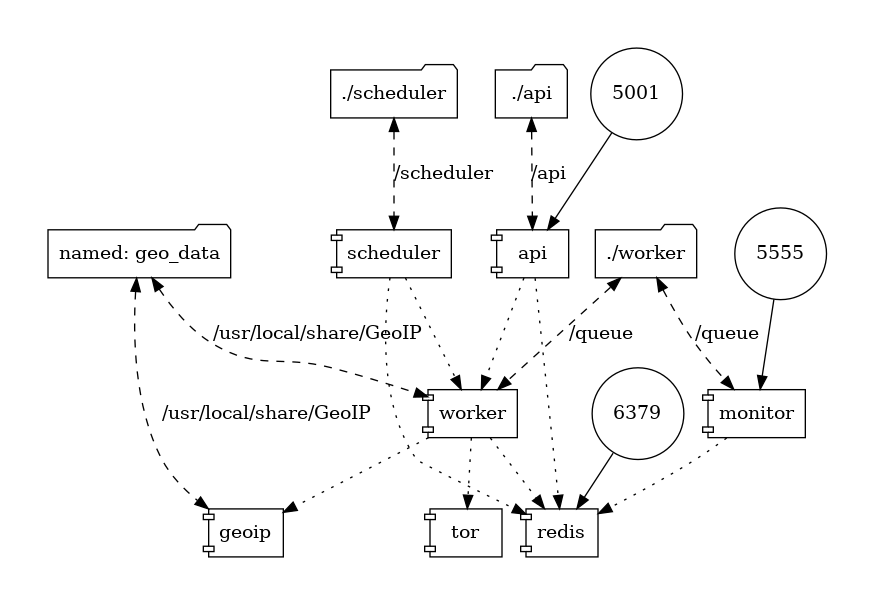
\includegraphics[width=0.75\linewidth]{graphs/docker-compose.png}
    \caption{Visualisation of VisiBot Docker-Compose Containers. Reverse Engineered using docker-compose-viz. Containers are represented as rectangles and exposed container ports as circles.}
    \label{fig:docker_graph} 
\end{figure}



% =========================================


\section{VisiBot Processing System}

\subsection{Database Record Storage using MongoDB}

Developed by \citet{MongoDB}, MongoDB is a Document-Oriented No-SQL database with extensive cross-platform support, allowing for the storage of documents represented in JavaScript Object Notation (JSON), a highly supported human-readable standard format. The VisiBot Processing System uses MongoDB widely to manage and store complex, and in some cases, nested, data objects through MongoEngine, an open-source python object data mapper for MongoDB \citep{MongoEngine}. As Documents are represented in a standard JSON format, database entries can be easily created, managed, and accessed by mapping MongoDB documents to standard Python objects and types, such as dictionaries and lists. Additionally, as this file format is widely accepted by various other programming languages, libraries/frameworks, and software applications, data collections stored within MongoDB Documents can be easily imported/exported, manipulated, and analysed by various popular data science, analytics and visualisation libraries.

Like relational databases such as PostgreSQL and MySQL, entity relationships of various cardinalities can also be established within MongoDB. However, unlike traditional relational databases, associations such as One-to-One and One-to-Many can be represented using embedded MongoDB documents (JSON Objects). This allows for the nesting of documents such that relational attributes are easily accessible and represented logically. Additionally, MongoDB allows for representing One-to-Many relationships by creating and referencing primary keys attributes through document reference fields. VisiBot uses such relationships, enabling the linkage of documents containing information for botnet IP addresses, Autonomous Systems, malware analysis reports, and more. A complete Entity Relationship diagram of all of the VisiBot Processing database is shown in Appendix \ref{appendix_a1}.

All data collected by the VisiBot Processing System is securely stored, managed, and accessed through a remotely accessible instance of MongoDB hosted through the MongoDB Atlas \citep{MongoDBAtlas}.

\subsection{Honeypot Data Collection}

All honeypot information processed by VisiBot is provided by \citet{BadPackets}, a leading provider of Cyber Threat Intelligence information on emerging threats, DDoS botnets, and network abuse. The honeypots hosted by Bad Packets are strategically deployed across a diverse set of network providers based in multiple countries and regions, including Australia, Brazil, Canada, France, Germany, India, Japan, Netherlands, Russia, Singapore, Taiwan, The Middle East, the United Kingdom, and the United States. Such honeypot servers are configured to emulate commonly targeted hosts specific to botnet traffic by mimicking various IoT devices, consumer-grade routers, enterprise VPN endpoints. Additionally, sinkhole domains previously used by threat-actors are employed to point potential botnet traffic to the honeypots.

Accessible through an authenticated REST API, the Bad Packets honeypot service is queried on an hourly basis from within a containerised task scheduler application written in Python. Using the python \texttt{requests} library \citep{PythonRequests}, the Bad Packets API is repeatedly accessed for honeypot packet results. Each result is converted into a Python dictionary and is appended to a list containing all results. An example Bad Packets honeypot result is shown in Appendix \ref{appendix_a2}.

Once all results within the last hour have been collected, the scheduler connects to the VisiBot Celery broker (Redis), hosted within a neighbouring docker container, and begins to create a Celery analysis task for each packet result. Task creation is requested through the client executing \texttt{Celery.send\_task}, passing the task name as a string and the result dictionary for analysis as an argument. Following this, tasks are created as pending messages within the broker and are actively consumed (executed) by available Celery workers. Once task creation has completed, the scheduler will wait until the next hour before extracting more results from Bad Packets, as new packet data is made available through the API at the beginning of every hour. All Celery can be viewed in the Flower web dashboard hosted from within a separate docker container:

\begin{lstlisting}[caption={Example output of VisiBot Processing Scheduler.}]
VisiBot collection event activated. Collecting data from Bad Packets API.
Querying Bad Packets (last seen after 2021-03-01T21:00:00Z)
Queried 927/927 results
Creating processing tasks for 927 results.
Workers are now running tasks in the background. Visit http:/flower:5555 to view progress.
\end{lstlisting}

Upon receiving a task from the broker, a Celery worker will perform an analysis of the received packet data. As the analysis procedure involves actively reading and writing from a database, each worker is configured to execute at most one concurrent job from the broker at any given time to avoid database connection locks. The honeypot packet analysis process is separated into multiple stages, spanning from malware payload URL extraction and traffic classification to sandbox analysis initialisation. 

\subsection{Malware payload extraction}

As previously discussed, when a device is infected with botnet malware, it will begin to scan for open ports of vulnerable devices and will attempt to infect such devices by sending malicious HTTP requests that contain command-line injection code. The injected code, also known as a Remote Code Execution attempt, will likely try to download and execute a malware binary using command-line utilities such as \texttt{wget}, \texttt{curl}, or \texttt{tftp}. Such exploit attempts are commonly found within the \texttt{payload} or \texttt{post\_data} of an offending packet. By extracting the URL of the botnet malware payload, the binary can later be retrieved, executed, and analysed. 

\subsubsection{Noise removal and de-obfuscation}

The first stage of malware payload extraction involves the removal of noise and elimination of the various obfuscation attempts employed by botnet developers. Due to the high number of different devices being targeted and exploits used, the structure and syntax of the command-line injection code captured by honeypots can vary significantly. Consider the following payloads strings:

%TC:ignore
\begin{lstlisting}[escapechar=@, caption={Example of noisy and obfuscated botnet payloads. Examples of noise are highlighted in \textbf{bold}, and obfuscation in \textit{italics}.}]
GET /language/Swedish${@\textbf{IFS}@}&&cd${@\textbf{IFS}@}/tmp;rm${@\textbf{IFS}@}-rf${@\textbf{IFS}@}*;wget${@\textbf{IFS}@}
http://[redacted_ip]:54134/Mozi.a;sh${@\textbf{IFS}@}/tmp/Mozi.a&>r&&tar${@\textbf{IFS}@}/string.js HTTP/1.0

GET /shell?cd /tmp; cp /bin/busybox yeet; >yeet; chmod 777 yeet; nohup wget
@\textit{http:/\textbackslash/}@[redacted_ip]:80/arm7 -O yeet || @\textit{nohup tftp -r arm7 -g [redacted\_ip] -l yeet}@;
chmod 777 yeet@\textbf{;./}@yeet Windows; rm -rf yeeter >/dev/null 2>&1 HTTP/1.1
\end{lstlisting}
%TC:endignore

As shown above, the first payload contains a lot of noise. The \texttt{\$\{IFS\}} variable is used as an input field separator in place of space characters. The second payload contains some light obfuscation employed to prevent regular expression patterns from matching URLs in the payload string. The first payload URL downloaded using \texttt{wget} has an escaped forward slash such that the pattern \texttt{http://} cannot be matched. Should the infiltrated system not have \texttt{wget} installed, the injected code also tries to download the binary using the \texttt{tftp} client. However, the malware payload URL is obscured using various command-line arguments, as the host of the URL is specified using the \texttt{-g} flag, the path using the \texttt{-r} flag, and the output using \texttt{-l}. These URLs can be re-built, but the presence of noise such as \texttt{\$\{IFS\}}-based spacing can make this process difficult. A shortlist of noisy characters and sub-strings is created through the manual inspection of several payload strings and post\_data contents. The list is used throughout the cleaning process, removing any significant noise from both the payload and post\_data packet strings. Each string is decoded such that any URL encoded values, such as \texttt{\%20} spacing, are converted into plain text. Similarly, occurrences of the sub-string \texttt{\$\{IFS\}} are replaced with space characters, and the removal of inconsistent spacing before/after command-line semi-colon separators (\texttt{;}) is also implemented. Lastly, the removal and/or replacement of the characters \texttt{\textbackslash"'`\&|()+} ensure that all URLs and \texttt{wget/curl/tftp} commands are clean.

\subsubsection{Payload URL extraction and validation} 

Following the removal of noise, both the payload and post\_data strings are combined into a string which is parsed for payload URLs using several techniques. A conventional URL regular expression pattern is used to match all un-obfuscated URLs contained within the payload strings. However, as this expression matches all sub-strings that begin with \texttt{https?://}, a large proportion of partial or obfuscated payload URLs will not match this regular expression. For example, consider the following sub-strings:

\begin{itemize}
    \item \texttt{curl website.com/bin;}
    \item \texttt{wget 127.0.0.1:8080/bin;}
    \item \texttt{tftp -g 127.0.0.1:8080 -r bin;}
\end{itemize}

Due to Regular Expression matching limitations, the extraction process also utilises other methods of URL extraction. The python library \texttt{urlextract} \citep{URLExtract} partial URL strings containing domain names, such as \texttt{website.com/bin}, by matching any occurrences of Top Level Domains (TLD), such as \texttt{.com, .net} and \texttt{.org}, until a stop-character, such as white space, is reached. This method allows for the extraction and validation of domain names used for botnet propagation, as partial domain-based URL strings are identified and re-formatted using the standard HTTP URL format. As these strings do not indicate a URL schema, the \texttt{http://} schema is used by default.

The practice of obfuscating payload URLs through executable arguments was frequently commonly observed across inspected honeypot payload command-line injection strings, as shown in the example sub-strings above. However, the VisiBot Processing System is capable of performing the automatic re-construction of argument-based obfuscated URLs, particularly from data-transfer command-line tools such as \texttt{curl, wget} and \texttt{tftp}. A utility function is used to identify the position at which commands such as \texttt{wget}, \texttt{curl}, and \texttt{tftp} are called, and the arguments following the start of the command are parsed until an end-of-line semi-colon (\texttt{;}) character is reached. Depending on the type of retrieval command, the function will look for and parse the contents of specific command-line arguments in order to extract the \texttt{host}, \texttt{port} and \texttt{path} of the obfuscated URL. For example, the helper function may identify usage of the \texttt{tftp} command and will extract the values passed within the \texttt{-g} and \texttt{-r} arguments, extracting the host, port, and path of the payload URL from the payload command-line injection string. Once extracted, the base URL is re-built through formatting extracted host, port, and path values within a standard http URL format: 

\begin{lstlisting}
url = "http://{host}:{port}/{path}".format("127.0.0.1", 8080, "bin")
>>> "http://127.0.0.1:8080/bin"
\end{lstlisting}

Following this step, GET requests are sent to each URL. The response data is parsed to identify if the URL leads to a binary executable, bash script, or non-executable file. All HTTP requests are routed through a Tor Proxy server hosted in a separate docker container from the celery workers for anonymity. All Non-executable URLs are disposed of, and identified binary executables are immediately added to the list of URLs awaiting validation. Binary execution is identified by checking if the HTTP request's content-type header begins with \texttt{application/}, or the contents of the request contains an Executable and Linkable Format (ELF) header. However, a current limitation is that botnet propagation bash scripts used in Remote Code Execution attempts cannot be executed within the LiSa sandbox environment. To combat this constraint, the worker will parse the contents of any bash script URLs and extract and store any nested URLs. Bash scripts often include links malware for various architectures, leading to VisiBot effectively extracting up to 6 (or more) binaries from a single bash script. Bash scripts are identified by checking if the header content-type starts with \texttt{text/} and the content of the request contains any of the following sub-strings: \texttt{["\#!", "wget", "curl", "tftp"]}. The first sub-string, \texttt{\#!}, represents a shebang character sequence read by Unix-based operating systems to indicate which interpreter should be used when executing a bash script \citep{Shebang}. For an example of a multi-binary bash script used for botnet propagation, see Appendix \ref{appendix_a3}.

Upon collecting all malware binary URLs, the Top Level Domain (if present), IP address, and host corresponding of each URL is further validated before proceeding with malware binary analysis. Using python libraries \texttt{tld} and \texttt{tldextract} \citep{TLD, TLDExtract}, the Top Level Domain of each URL is extracted and checked against a list of ignored TLDs, including \texttt{.gov, .mil} and \texttt{.arpa}. The host-name and IP address of each URL are identified using the built-in python \texttt{socket} library. \citep{PythonSocket} Once identified, the URL, host-name and IP address are used to create a new \texttt{MalwarePayload} database entry. If an instance of the URL already exists, its corresponding entry is updated, and the URL is dropped from the list of URLs awaiting malware analysis. When creating an entry, the worker will determine if the malware payload is self-hosted by the source IP address attempting to infect the honeypot by matching the packet's source IP address with the IP address identified from the extracted URL. 

\subsection{Botnet traffic classification}

Following the extraction of URLs from a given honeypot packet, the worker will infer the classification of both the source and payload IP addresses based on the context of the extracted URLs and the command-line code injection string's contents. If one or more URLs is successfully extracted and at least one URL is self-hosted by the packet's source IP address, the worker will classify the source/payload IP address as a "Malicious Bot". Bad actors use malicious Bots to self-propagate botnets without the need for an external payload server. Malware binaries are downloaded onto the infected machine and used as a download host when infecting other devices.

If the IP address of the payload URL does not match the source IP, the payload host is classified as a "Payload Server", and the source IP address is classified as a "Report Server". As seen in botnet variants such as Mirai, as infected bots scan for vulnerable devices, they will report such findings to a report server. The report server will attempt to infect the device through command-line injection, using malware remotely hosted on a separate payload server. For simplicity, both infected hosts and report servers that attempt to infect devices using malware hosted on payload servers are classified as report servers.

Alternatively, if no URLs are extracted from the honeypot packet payload or post\_data strings, the worker will use additional information provided by the Bad Packets API to determine if the packet contains characteristics representative of passive botnet activity, such as port scanning. By monitoring packets received by honeypots, all packets are evaluated in terms of target port usage and payload exploit characteristics to identify various Common Vulnerability Exploit (CVE) tags and descriptive categories such as "Mirai-like scan". Bad Packets detect Mirai-like scans by analysing the TCP sequence number of a given packet and checking if it is equal to the targeted device's IP address, as shown in the Mirai source code snippet shown below. \citep{BadPacketsMirai}

\begin{figure}[!htb]
    \centering
    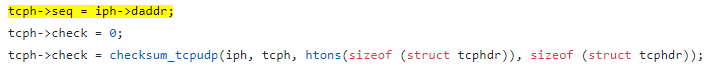
\includegraphics[width=0.75\linewidth]{images/mirai-like-signature.png}
    \caption{Mirai TCP sequence source-code. Snippet provided by \citet{BadPackets}}
    \label{fig:mirai_like_scan} 
\end{figure}

Using the additional tag information provided by Bad Packets, VisiBot can infer if a packet is associated with botnet scanning activity. Any honeypot packet that does not contain a payload URL is classified as 'Bot' if it demonstrates either Mirai-like or general port scanning activity, which is determined based on its TCP signature or target port.  

\subsection{Honeypot Packet Processing}

Following the identification and classification of a packet's source IP address (and any associated payload servers), additional IP address metadata is collected using various heterogeneous data sources. The geographic information for each classified IP address is looked up using locally hosted MaxMind GeoIP2 databases \citep{MaxMind}, which is then stored in the database for future use. Such information includes the latitude and longitude, city, country, and the continent of a given IP address. Privacy and hosting information for a given IP address is also identified using the IPInfo Privacy Detection API \citep{IPInfo}, allowing for identification of servers provided by hosting services and the detection of a Proxy, VPN, or Tor service. Lastly, Autonomous System history information is collected using the \texttt{ipwhois} python module. This module performs an IP WHOIS lookup for a given address and returns Autonomous System information sourced from Internet Service Registries including AFRINIC, APNIC, and RIPE NCC \citep{Afrinic, Apnic, RipeNCC}.

Following the IP address metadata collection, a new event log entry is created for each IP address. Each entry indicates the event classification label and the time and date of occurrence. Additionally, all relationships between a given packet's source IP address and payload IP addresses are stored within the database. IP address connections are specified by including the IP addresses of the source and destination of a connection and a 'last seen' timestamp. Lastly, the packet JSON data sourced from the Bad Packets honeypot service is also stored directly within the VisiBot database. Each record contains valuable information for botnet analysis, including the targeted port, request user-agent, Bad Packets tags, and event count. To visualise the overall structure of the VisiBot database, please refer to the entity-relationship diagram shown in Appendix \ref{appendix_a1}.

Following the above steps, the VisiBot worker will continue by iterating over the list of extracted payloads URLs and sequentially send an analysis task creation HTTP request to a remotely hosted malware sandboxing service. Within each API request, the worker specifies the URL for analysis and the execution time in seconds, with a default of 30 seconds. Following the successful creation of each malware analysis task, the sandbox server will respond with a unique \texttt{task\_id} identifier, which is stored within the VisiBot database alongside the ID of the payload being analysed. Upon analysis completion, the sandboxing server will send an analysis report to the VisiBot Processing System through a REST API, which is further analysed for candidate botnet Command \& Control server and Peer-to-Peer node identification. A complete low-level overview of the VisiBot Processing System is shown in Appendix \ref{appendix_a4}.

\subsection{LiSa Sandbox Integration}

Developed by Daniel Uhříček, the LiSa Sandbox \citep{LiSa} is an open-source, scalable, and automated Linux Sandbox platform. It supports the execution and analysis of malware binaries compiled to various CPU architectures, including MIPS, ARM, x86\_64, i386, and aarch64. Like the VisiBot Processing System, LiSa is also a multi-container docker application. It invokes the message-broker design pattern using Celery and RabbitMQ as message broker \citep{Celery, RabbitMQ} and is accessible through both a web dashboard and REST API. By default, the LiSa sandbox allows for remote static and dynamic analysis of binary executables but can be extended to include additional analysis stages. The number of workers used to analyse binaries can be scaled in the same way VisiBot workers are scaled, using the \texttt{-scale worker=N} argument when starting the service using \texttt{docker-compose}. This allows for easy distribution of analysis tasks, enabling multiple binaries to be processed at a given time. 

Static analysis information is directly extracted from uploaded binaries using Radare2 \citep{Radare2}, a comprehensive binary analysis framework, allowing for the identification of a given malware binary's target CPU architecture, endianness, operating system, and more. Dynamic and network analysis are performed through the direct execution of a malware binary within a sandbox environment. Each binary is executed within the QEMU virtual machine \citep{Qemu} using an embedded Linux image that matches the detected binary CPU architecture. As LiSa supports five different architectures, an embedded Linux image has been created for each architecture using Buildroot \citep{Buildroot}. If an unsupported architecture is detected, the task will purposefully fail, and the payload will be processed by VisiBot accordingly. A variety of dynamic analysis information is logged during execution, including packet data, machine log information, process trees, system calls, opened files, and program output. Using the collection of static and dynamic data collected, LiSa generates a report for each malware analysis task which contains network analysis information such as IP address endpoints, HTTP requests, DNS queries, telnet data and IRC messages. Users are also given the option to provide an API key for automatic aggregation of various anti-virus scanning services through VirusTotal \citep{VirusTotal}. As the VirusTotal scan reports of identified malware binaries are actively used throughout VisiBot analysis, this service was facilitated using an academic VirusTotal API key.

\subsubsection{Modifications to LiSa}

Despite the extensive feature-set provided by the default LiSa sandbox configuration, some limitations were encountered when integrating the sandbox into the VisiBot Processing System. Several modifications were made to the LiSa sandbox source code via a public GitHub fork \citep{LiSaModified} to mitigate such issues. A significant issue was that binaries had to be provided as file attachments by default when creating analysis requests through the LiSa REST API, meaning VisiBot would first have to download binaries before uploading them to LiSa. As this is not ideal, the LiSa sandbox API has been modified to accept an additional \texttt{url} parameter for the URL of a binary to be provided instead of the file itself, mitigating any security issues presented by downloading malware directly onto the VisiBot server.

Several malware binaries were observed to have been packed using packing software to obfuscate source code strings extracted during the LiSa static analysis process. Any attempt to extract strings from a packed malware binary would result in unreadable, compressed, and thereby heavily obfuscated output. Malware authors incorporate binary packing as a means of additional obfuscation, as packed binaries often contain strings such as IP addresses. These binaries are unpacked into the program's address space at run-time, \citep{Roundy2013} ensuring that analytical software tools, such as the \texttt{strings} command-line tool \citep{Strings} used by LiSa, output nonsensical information. Modifications were made to the LiSa sandbox to enable the automatic detection and unpacking of malware samples using the UPX packing tool \citep{UPX}. UPX a popular tool used for obfuscating the contents of Linux/Unix executables. This tool leaves an identifier signature in the strings of a packed malware, allowing for quick identification when parsing the output of the \texttt{strings} command executed by the LiSa analysis worker. If the substring "UPX!" is found in the strings of a binary, the worker will attempt to unpack the binary using the command \texttt{upx --decompress path/to/file}. Following this, the string values of the unpacked binary are collected by re-running \texttt{strings} on the binary.

Lastly, when integrating the LiSa sandbox with the VisiBot Processing System, various communication-based limitations were encountered. As the LiSa sandbox's source code only allows for one-way communication through a REST API, there was no efficient way for the VisiBot Processing System to detect when analysis tasks were complete. An initial solution was to repeatedly query the LiSa API for task status updates, yet this proved highly inefficient and ultimately introduced several reliability issues. Thus, the VisiBot Processing System hosts a minimal REST API written in Flask, \citep{Flask} used by LiSa sandbox workers to send back completed analysis tasks. Adding a REST API to the processing system allows for a robust two-way communication system between VisiBot and the LiSa sandbox server.

Hosted within a separate docker container, the VisiBot Flask API accepts two types of HTTP request from the LiSa Sandbox via the endpoints \textit{/api/lisa-analysis/success/<task\_id>} and \textit{/api/lisa-analysis/failure/<task\_id>} respectively. Additional modifications have also been made to the LiSa sandbox such that success/failure reports are sent back to the VisiBot API following task completion. If an analysis task succeeds, LiSa will send the malware analysis report back to the VisiBot Processing System for further analysis. Whereas, if an analysis task fails, stack trace information is returned to VisiBot to handle failed payloads. Responses are handled by creating corresponding Celery tasks, which are eventually consumed and carried out by available VisiBot workers. Failed tasks are processed based on the type of exception generated during analysis. For example, if a \texttt{UnicodeDecodeError} was raised, this indicates that the extracted payload URL points to a non-executable file. Thus, the MalwarePayload document (and all other related documents) is removed from the MongoDB database.

\subsection{Malware Analysis Information Extraction}

Before applying identification heuristics, the worker will first attempt to parse the top-most recurring malware keyword from an aggregated list of anti-virus vendor scan results via VirusTotal. However, many anti-virus vendors do not follow the same naming convention when labelling the type of malware detected. Thus, additional steps are taken to standardise the keyword extraction process by removing punctuation, case sensitivity, and generic keywords such as \texttt{Trojan, Malware, Worm}, etc. What remains is a list of unique keywords used by vendors to characterise the type of malware detected. The most commonly recurring keyword across all vendor results is used as the primary keyword identifier for the analysed malware. For an example of this process, please refer to Appendix \ref{appendix_a5}.

Following keyword extraction, the worker will parse each of the binary strings collected during the static analysis stage of the LiSa sandbox analysis, such that any strings of significance, such as IPv4 and IPv6 addresses, URLs, and domains, are extracted using regular expression. As storing the entire list of malware strings proved too memory consuming, this step was necessary to reduce the amount of unnecessary data stored within the database.

\subsection{Application of heuristics}

Using the malware analysis report generated by LiSa, any significant network traffic, such as that of candidate Command \& Control Servers and possible Peer-to-Peer botnet nodes, is detected through the direct application of the following four heuristics. Each heuristic is applied to the static or network analysis information confined within the report for a given malware sample to infer if the host running the malware has actively communicated with external botnet entities. The four heuristics applied throughout the heuristic analysis process are as follows:

\begin{enumerate}[i]
    \item The infected host performs a Peer-to-Peer DNS Query during network analysis.
    \item The infected host performs a data transaction with a foreign IP address.
    \item Interaction detected between the infected host and hard-coded IP address.
    \item Interaction detected between the infected host and blacklisted Command \& Control Server IP address.
\end{enumerate}

\subsubsection{Heuristic (i)}

As inferred by its description, the first heuristic is primarily used to distinguish between centralised and de-centralised botnets through identifying a common Peer-to-Peer botnet characteristic. By analysing the DNS queries performed by a given malware sample during sandbox analysis, we can infer that the malware communicates through Peer-to-Peer networks if any of the domains fall within a known list of DNS names associated with known Peer-to-Peer services. As de-centralised botnets often use Distributed Hash Tables as a means of communication between peer botnet nodes, a device infected with peer-to-peer botnet malware may attempt to look up a distributed hash table using a common BitTorrent service. For example, a botnet may query the domain \textbf{dht}.bittorrent.com as part of the distributed hash-table lookup. Thus, all DNS queries are compared against a shortlist of BitTorrent domain name wildcards commonly used by Peer-to-Peer botnets:

\begin{itemize}
    \item \texttt{.utorrent.com}
    \item \texttt{.transmissionbt.com}
    \item \texttt{.bittorrent.com}
    \item \texttt{.debian.org}
\end{itemize}

If any of the above domain patterns are matched, the system assumes that the incoming traffic is likely associated with a Peer-to-Peer botnet, hence, the heuristic \textit{i)} is satisfied. However, as this heuristic only indicates Peer-to-Peer network activity, it cannot be used exclusively for Peer-to-Peer botnet identification. Instead, it must be used in conjunction with heuristic \textit{ii)} to infer if the traffic is that of botnet activity.

\subsubsection{Heuristic (ii)} A data transaction may occur during network analysis of a malware binary when the infected host sends a series of bytes to an external IP address and receives a stream of bytes in response. This activity may include hand-shakes or communication between an infected host and C2 server, downloading a binary from a remote Payload Server, or interactions between peer-to-peer botnet nodes. Thus, this heuristic allows for the distinction between benign and potentially malicious network traffic. IP addresses that actively send and receive information to/from an infected host (i.e. endpoints which participate in a data transaction) will satisfy this heuristic. If both heuristics \textit{i)} and \textit{ii)} are satisfied, it is concluded that the corresponding IP address \textit{ii)} may be a potential peer-to-peer botnet node. However, if only heuristic \textit{i)} is satisfied, it is inferred that the IP address may be a potential (candidate) Command \& Control server. Notably, this classification will consider any data transactions between an infected host and a Payload server as possible C2 activity, as the botnet owner may also use the Payload Server for Command \& Control.

\subsubsection{Heuristic (iii)} As it is common for centralised botnet malware to include hard-coded IP addresses and domains used for C2 communication, the heuristic \textit{iii)} infers that any IP address logged during network analysis that is contained within a list of hard-coded IPv4 addresses from the binary's source may be a potential Command \& Control server. All endpoints are checked against a list of hard-coded IPv4 strings extracted from the previous stage of the LiSa analysis process. If any match occurs, then the heuristic \textit{iii)} is satisfied, and the IP address will be classified as a candidate Command \& Control server.

\subsubsection{Heuristic (iv)} If any IP address connections are logged during the network analysis as known blacklisted Command \& Control servers, the heuristic \textit{iv)} is satisfied. The VisiBot Processing system checks the blacklist status of each IP address endpoint encountered during malware analysis by performing lookups across various IP blacklist services, including those provided by Barracuda Central, abuse.ch, SpamRats, Sorbs DNSBL, and Spamhaus. \cite{BarracudaCentral, AbuseCh, Spamrats, SorbsDnsbl, SpamhausZen} If any IP address has previously been blacklisted as a C2,  the IP address is classified as a candidate Command \& Control server.

Following heuristic botnet analysis, each IP address is classified either as a candidate C2, a Peer-to-Peer Node, or benign traffic (which is ignored). Candidate C2 or P2P entries are added to the VisiBot database if any of the heuristic requirements are satisfied. A variety of additional IP address metadata is also collected, as previously performed in the packet analysis stage. New botnet event logs are also stored, and IP address connection records are created/updated between the associated payload IP and all C2/P2P IPs encountered during analysis. Lastly, the LiSa analysis report is refined to include only essential information and is stored within the database along with any significant strings extracted during the analysis process. Once this stage is complete, the worker will continue to process other tasks by consuming a new analysis task from the VisiBot broker queue.

% =========================================


\section{Interactive Web Visualisation}

A map-based web application is created to provide an interactive visualisation of all botnet traffic detected by the VisiBot Processing System within a 24-hour window. The web application was designed and implemented following the Model View Controller (MVC) design pattern, as the development of the front-end presentation layer and back-end data interaction layer are independent, allowing for a separation of concerns. The model layer used is the same MongoDB data store \citep{MongoDB} utilised by the VisiBot Processing System. Users can interact with various aspects of the model through a front-end visualisation layer written in the Nuxt.js \cite{NuxtJS} JavaScript framework, which communicates with a back-end web API created using Express.js. \citep{ExpressJS} Express is a flexible web application framework written in Node.js, \citep{NodeJS} which is used as a controller interface between the database and front-end application:

\begin{figure}[!htb]
    \centering
    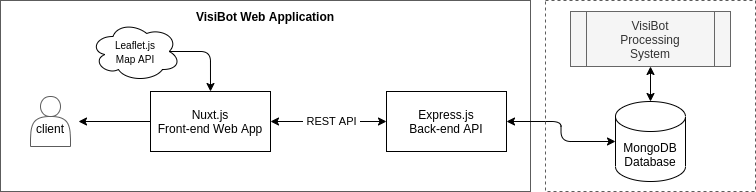
\includegraphics[width=0.75\linewidth]{flowcharts/frontend_flow_diagram.png}
    \caption{Server Architecture Diagram: VisiBot Web Application}
    \label{fig:frontend_server_architecture} 
\end{figure}

The back-end Exprss.js REST API communicates with the VisiBot MongoDB database using Mongoose, an Object Data Modelling (ODM) library for MongoDB. \citep{Mongoose} Upon a client sending an HTTP request to the API, the Express.js server will query the MongoDB database directly using Mongoose and returns documents to the client in the standard JSON format. As Express, Mongoose, and Nuxt.js are JavaScript-based, the JSON-based document structure used to represent MongoDB documents is natively supported across all three frameworks, allowing for extensive flexibility without introducing overhead such as JSON serialisation. In conjunction with Nuxt.js and Express.js, several \texttt{npm} packages were also used throughout development. The BootstrapVue \citep{BootstrapVue} library was used with Nuxt.js to develop a modern, flexible, and intuitive user interface using the Bootstrap CSS framework.

\subsection{Geographic Clustering and Networks}

An interactive, cluster-based map was developed using \citep{LeafletJS} to allow for real-time interaction with the various botnet entities identified by the VisiBot Processing System. This map displays a clustered representation of the geographic locations of all entities identified within the last 24 hours, with each IP address displayed as a coloured marker. The colour of the marker depends on the classification of traffic coming from the IP address. As the user zooms in on the map, the clusters dynamically become smaller in size, allowing for the user to interact with the full extent of the map without experiencing information overload or the performance side-effects of displaying too many markers at once. An example of the VisiBot Web Application interface is shown below:

\begin{figure}[!htb]
    \centering
    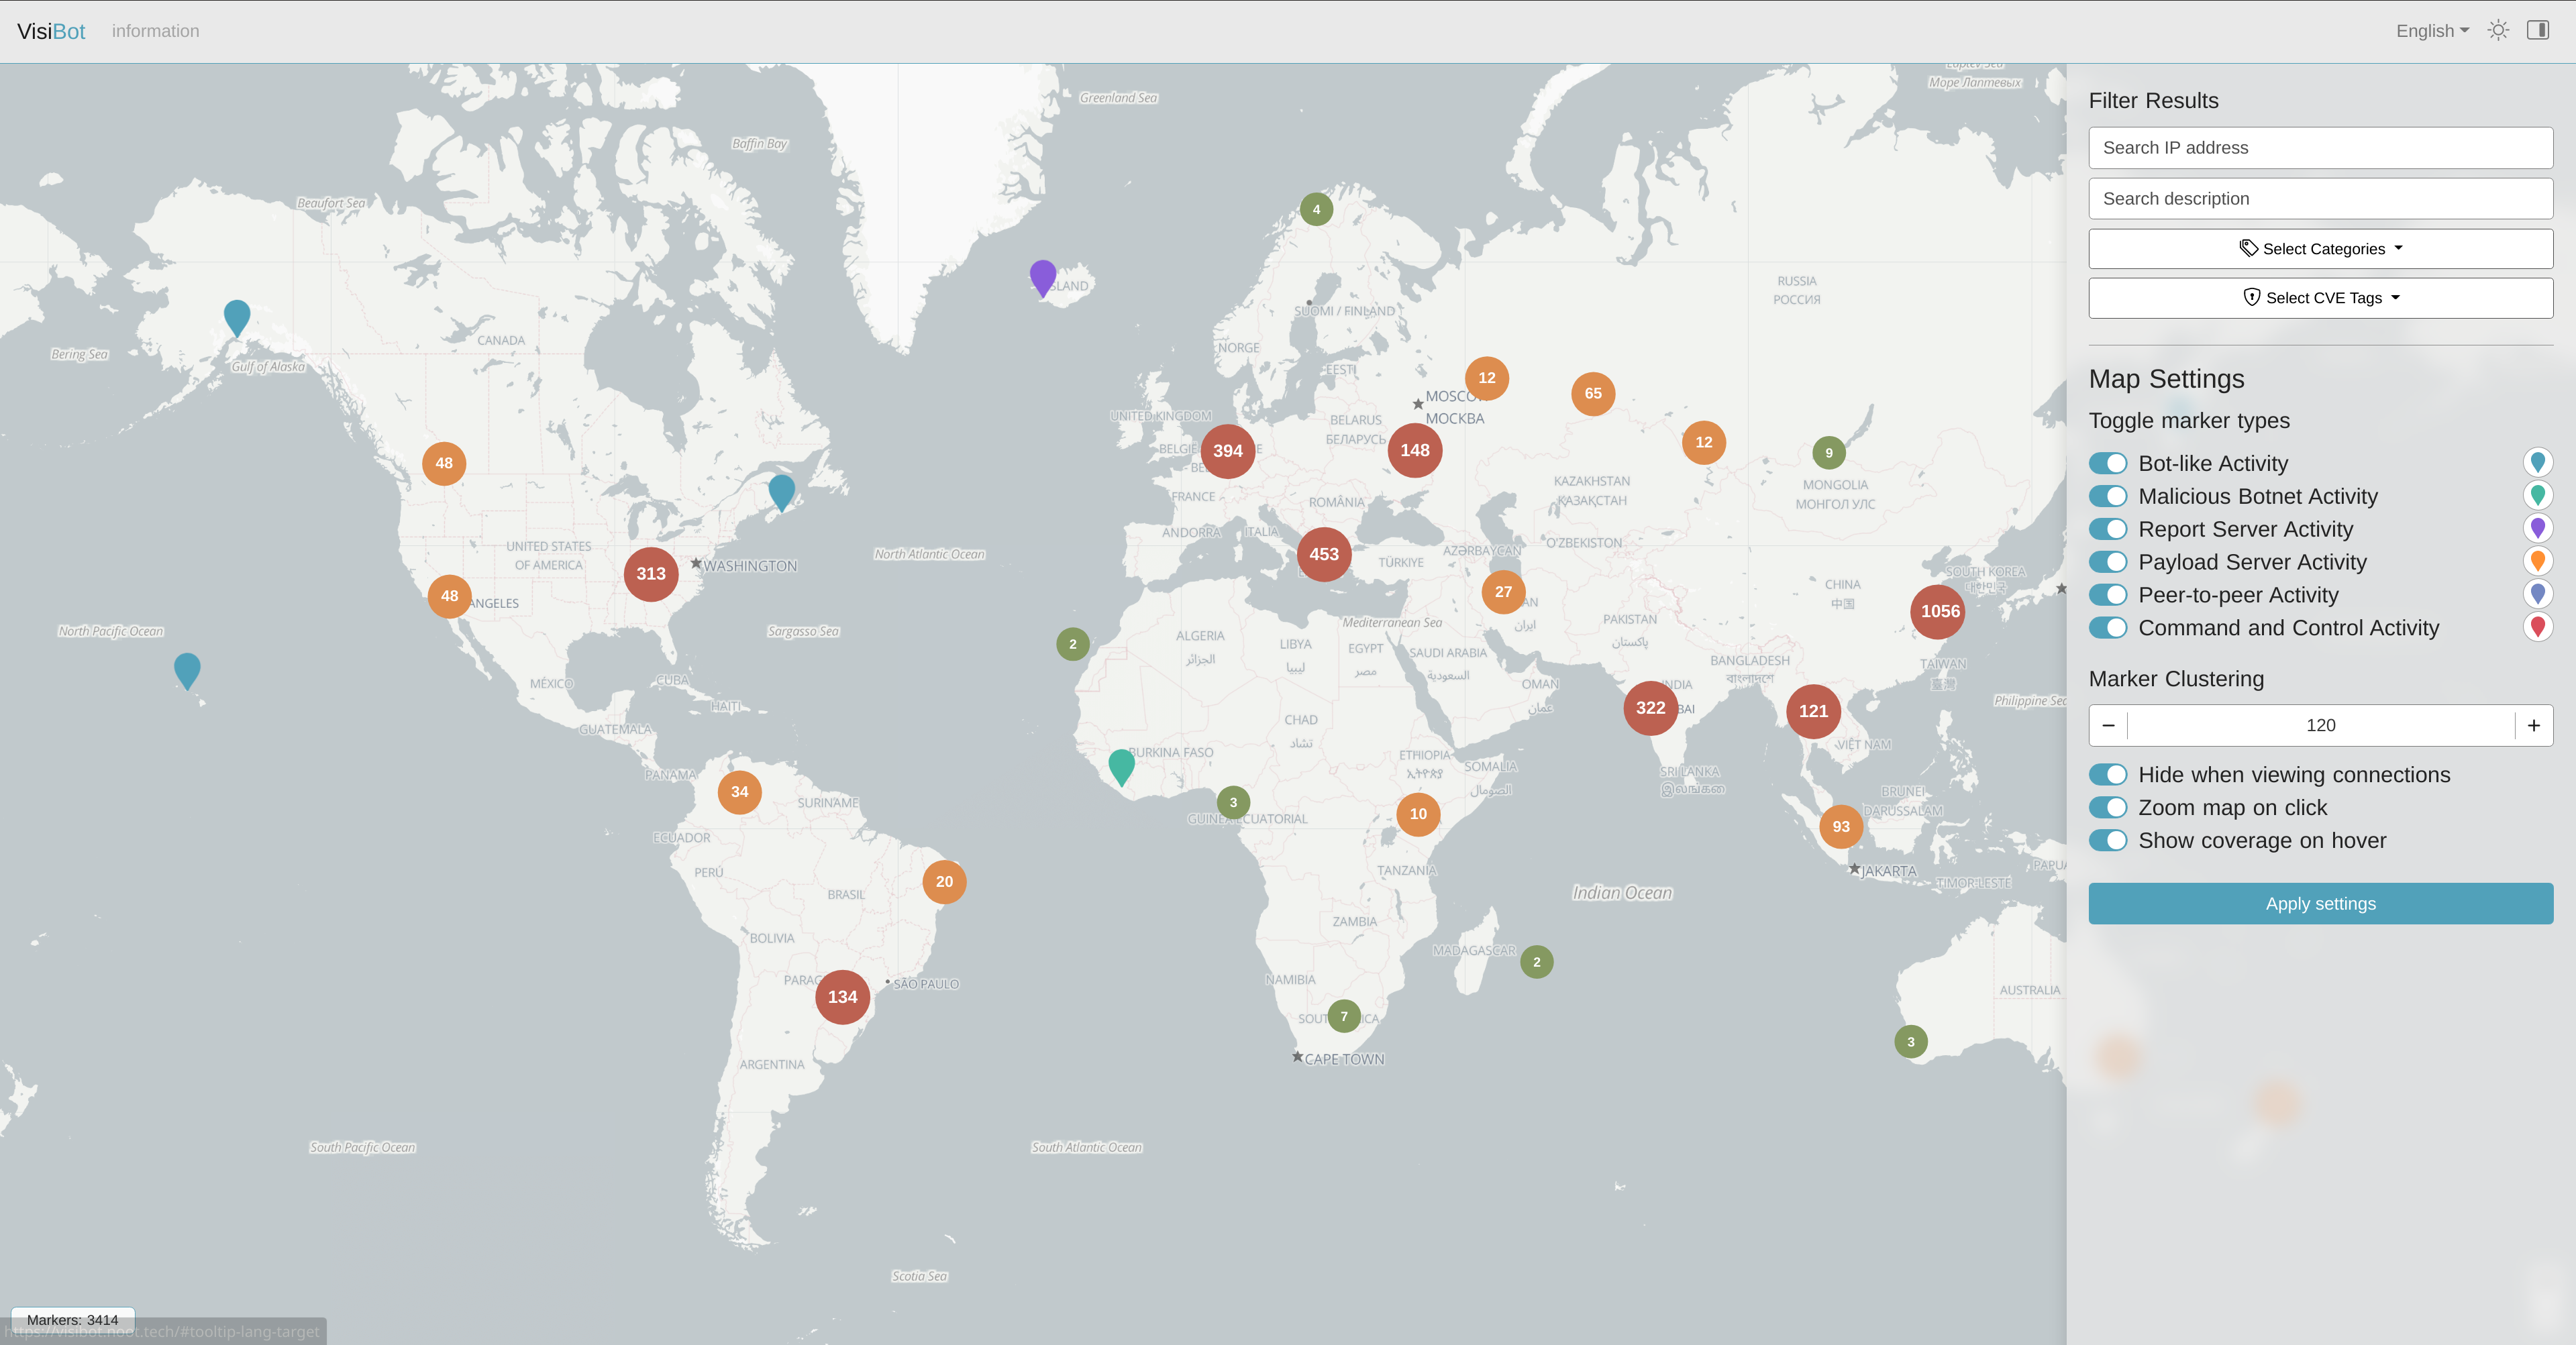
\includegraphics[width=0.8\linewidth]{images/visibot_screenshot_cluster.png}
    \caption{VisiBot Web Application}
    \label{fig:visibot_screenshot_cluster} 
\end{figure}

When a cluster is selected, the map will automatically zoom in and disseminate the clustered markers into smaller clusters or individual markers, depending on the cluster density. When a marker is selected, the user is presented with three options. The first option allows the user to view a network of all of the associated connections that the current IP address has with other botnet entities identified by VisiBot. For example, a candidate C2 server's connections may include interactions with payload servers, report servers, or infected bots. These connections are generated using the \texttt{graphLookup} document aggregation \citep{graphLookup} provided by MongoDB, allowing for full traversal of the connection tree of a given IP address. All coordinates collected using \texttt{graphLookup} for a given IP address are drawn as lines on the map, as demonstrated in the Peer-to-Peer connections example shown in appendix \ref{appendix_a6}.


% =========================================


\section{Software Development Practices}

\subsubsection{Issue Tracking}

Trello, a Kanban-style web-based ticket tracking application, was used throughout development to manage the various deadlines, priorities, tasks, and to-do lists.  As development tasks in Trello are represented as tickets, I managed my progress by sorting each task based on development status and priority. All tickets were actively moved between 'Backlog', 'In Progress', and 'Complete' columns, allowing me to keep track of the tasks I have yet to complete. Using a board-based ticket management system ensured I could manage my work without being overwhelmed by long to-do lists, as all tasks, priorities, and features are displayed in a highly coherent and user-friendly interface. More so, Trello also proved highly beneficial for tracking and managing various project-related deadlines and nested to-do lists, as each ticket can be assigned a due-date timestamp and is capable of encapsulating several sub-lists of tasks which can be updated using interactive check-boxes. 

\subsubsection{Quality Assurance}

Throughout development, linting tools and unit testing tools were used as a means of quality assurance. Several unit tests were written for the Bad Packets API using the unittest \citep{uniittest} python testing framework, ensuring reliable and robust code execution throughout the deployment of the project. Pylama, an auditing/linting tool for Python, \citep{pylama} was frequently used to ensure standardised coding style and readability. Pylama wraps various linting tools into a single code auditing tool, including popular linters such as Pylint, PyFlakes, and pycodestyle. The combination of various linting tools enables strict enforcement of various practices followed by Python programming professionals, including official style guides, such as the PEP-8 style guide written by \citet{PEP8}. Additionally, ESLint, \citep{ESLint} a static analysis linting tool for JavaScript, was also used for actively identifying problems in both Nuxt.js and Express.js web applications, including factors such as consistency, readability, and correctness. Both Python and JavaScript linting tools proved excellent for identifying an abundance of errors and inconsistencies amongst the VisiBot code-base, minimising potential issues that may have otherwise surfaced from inconsistent or poorly written code.

\subsubsection{Source Code Management}

All source-code managed using Git \citep{Git} version control and was also remotely hosted on a private repository using the GitHub \citep{GitHub} code-hosting and collaboration platform. Throughout the development of VisiBot, I strictly followed a trunk-based branching strategy such that all SCM changes were implemented as small, frequent commits to the master/main branch of the repository. As I was the sole developer throughout the implementation of VisiBot, branching strategies such as feature branching were considered unnecessary, as the likelihood of encountering merge conflicts within a single-developer work environment is highly unlikely. Before pushing any local changes to the remote repository, all code is automatically tested locally using Git pre-push hooks. \citep{PrePushHooks} By hooking a shell script onto the \texttt{git push} command, the contents of the script is executed and evaluated before the push request is processed. If the script exits with an error, the user must fix the errors raised during the pre-push script execution before allowing for changes to be pushed to a remote branch. Within the context of VisiBot, code linting and unit testing stages were automatically executed locally before pushing to a remote GitLab repository using a pre-push script. This script executes various unit tests, and the \texttt{pylama} and \texttt{eslint} linting tools within \texttt{src/processing} and \texttt{src/webapp} directories consecutively. By doing so, quality assurance is maintained by ensuring that if either of the linting tools or unit tests fail, the push request will be aborted until all issues are resolved. All unit testing and linting tools are also automatically performed through a Continuous Integration (CI) Pipeline deployed using the Travis CI \citep{TravisCI} Continuous Integration service. As TravisCI is integratable with GitHub, it was used throughout development to automate the linting and unit-testing quality assurance measurements whenever code is pushed to a monitored GitHub branch, such as the master branch. If the pipeline fails, all branch maintainers are alerted of the failure and are responsible for fixing any issues. The automatic testing of code ensures that even if a developer pushes code without testing locally, all code is tested before merging into the master branch.
